\newpage

\captionsetup{labelformat=empty}

\section*{\texorpdfstring{Appendix C: VOI for conservation auctions
heuristic solution \emph{n} =
2}{Appendix C: VOI for conservation auctions heuristic solution n = 2}}\label{appendix-c-voi-for-conservation-auctions-heuristic-solution-n-2}
\addcontentsline{toc}{section}{Appendix C: VOI for conservation auctions
heuristic solution \emph{n} = 2}

\textbf{Priors}

Let \(A_1\) and \(A_2\) be two assets. Each has some cost efficiency
\(c_1\) and \(c_2\), both of which are uncertain with prior probability
distributions,

\begin{equation}
c_1\sim\mathcal{N}(\mu_1, \sigma_1)
(\#eq:c1)
\end{equation}

and

\begin{equation}
c_2\sim\mathcal{N}(\mu_2, \sigma_2)
(\#eq:c2)
\end{equation}

where \(\mu_1\) and \(\mu_2\) are the prior means and \(\sigma_1\) and
\(\sigma_2\) are the prior standard deviations.

Let \(\pi=\Pr(c_1 > c_2)\) and therefore,

\begin{equation}
\pi = \Phi\left(\frac{\mu_1-\mu_2}{\sqrt{\sigma^2_1+\sigma^2_2}}\right)
(\#eq:c2)
\end{equation}

\textbf{Utilities}

If \(\pi > 1 - \pi\) then the optimal action is to purchase asset
\(A_1\), otherwise it is to purchase \(A_2\).

We can assign utilities to each combination of the condition of \(c_1\)
and \(c_2\), and each action such that,

\begin{equation}
\begin{aligned}
u(c_1 > c_2, A_1)&=1\\
u(c_1 < c_2, A_1)&=0\\
u(c_1 > c_2, A_2)&=0\\
u(c_1 < c_2, A_2)&=1\\
\end{aligned}
(\#eq:utilitiesapen)
\end{equation}

Therefore the expected values of taking each action are
\(\mathrm{E}[u(A_1)]=\pi\) and \(\mathrm{E}[u(A_2)]=1-\pi\).

\textbf{Value of perfect information}

If we could reduce the uncertainty in the prior probabilites of \(c_1\)
and \(c_2\) such that \(\pi\) approached either limit, then the expected
value of perfect information is,

\begin{equation}
\mathrm{EVPI}=1-\max(\pi, 1-\pi)=\min(\pi, 1-\pi)
(\#eq:evpiaucapen)
\end{equation}

\textbf{Preposterior analysis}

Now let's assume we can sample from some process and learn about \(c_1\)
and \(c_2\).\\
Let \(X_1\) and \(X_2\) be observations from a process described by the
following sampling distributions,

\begin{equation}
X_1\sim\mathcal{N}\left(c_1, 1\right)
(\#eq:x1)
\end{equation}

and

\begin{equation}
X_2\sim\mathcal{N}\left(c_2, 1\right)
(\#eq:x2)
\end{equation}

where for simplicity the standard deviation is one.

Furthermore, we can make \(Mp\) and \(M(p-1)\) observations of \(X_1\)
and \(X_2\) respectively. Where \(M\) is the total number of samples the
budget allows and \(p\) and \(p-1\) are proportions of that budget
allocated to each assets. Given the observations of \(X_1\) and \(X_1\)
with sample sizes \(Mp\) and \(M(p-1)\) we can update the prior beliefs
in \(c_1\) and \(c_2\) and arrive at posterior distributions,

\begin{equation} 
\begin{aligned}
c_1^\prime &\sim \mathcal{N}(\mu^\prime_1, \sigma^\prime_1)\\
c_2^\prime &\sim \mathcal{N}(\mu^\prime_2, \sigma^\prime_2)
\end{aligned}
(\#eq:posteriorcs)
\end{equation}

where,

\begin{equation}
\begin{aligned}
\mu^\prime_1 &= \frac{\mu_1 + X_1Mp\sigma^2_1}{Mp\sigma^2_1 + 1}\\
\sigma^\prime_1 &= \sqrt{\frac{\sigma^2_1}{Mp\sigma^2_1 + 1}}\\
\mu^\prime_2 &= \frac{\mu_2 + X_2M(p-1)\sigma^2_2}{M(p-1)\sigma^2_2 + 1}\\
\sigma^\prime_2 &= \sqrt{\frac{\sigma^2_2}{M(p-1)\sigma^2_2 + 1}}
\end{aligned}
(\#eq:posteriormusig)
\end{equation}

\textbf{Value of sample information}

Now we make the simplifying assumptions that
\(\mathrm{E}[X_1]=\mathrm{E}[c_1]=\mu_1\) and
\(\mathrm{E}[X_1]=\mathrm{E}[c_1]=\mu_1=0\).

In this scenario the prior probability of \(c_1>c_2\) is,

\begin{equation}
\pi=\Phi\left(\frac{\mu_1}{\sqrt{\sigma^2_1+\sigma^2_2}}\right)
(\#eq:priorpi)
\end{equation}

, and the posterior is

\begin{equation}
\pi^\prime=\Phi\left(\frac{\mu_1}{\sqrt{\frac{\sigma^2_1}{Mp\sigma^2_1 + 1}+\frac{\sigma^2_2}{M(p-1)\sigma^2_2 + 1}}}\right)
(\#eq:posteriorpi)
\end{equation}

We can now calculate the expected value of sample information,

\begin{equation}
\mathrm{EVSI}=\max(\pi^{\prime}, 1-\pi^{\prime})-\max(\pi, 1-\pi)
(\#eq:evsiaucapen)
\end{equation}

\textbf{Optimal sampling allocation}

With equations 10-12, for any given set of \(\mu_1\), \(\sigma_1\),
\(\mu_2\), and \(M\) we can find the optimal allocation to sample for
asset \(A_1\), \(p\) to maximise the value of sample information.

\textbf{Summary}

\begin{itemize}
\tightlist
\item
  Optimal allocation insensitive to ratio of \(\mu_a\) to \(\mu_b\).
\item
  Optimal allocation sensitive to ratio of \(\sigma_1\) to \(\sigma_2\).
\item
  Always preferential to sample asset with greater uncertainty.
\item
  Solution is symmetrical.
\item
  The \(M\) at which you start to allocate sampling to both assets is
  proportional to the ratio of \(\sigma_1\) to \(\sigma_2\).
\item
  The \(M\) at which you start to allocate sampling to both assets is
  insensitive to whether \(\sigma_1 < \sigma_2\) or
  \(\sigma_1 > \sigma_2\).
\item
  Optimal allocation always has greater EVSI when
  \(\sigma_1 \neq \sigma_2\).
\end{itemize}

\textbf{\(\mu_1 > \mu_2, \sigma_1 \gg \sigma_2\)}

First let's examine the case where our prior belief is that \(c_1\) is
somewhat greater than \(c_2\), where \(\mu_1=.2\) and \(\mu_2 = 0\) but
the uncertainty in \(\theta_1\) is far greater than in \(\theta_2\),
\(\sigma_1 = 2\) and \(\sigma_2 = .2\).

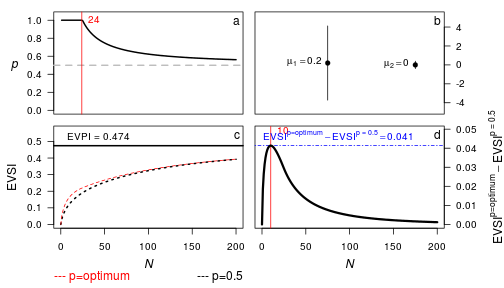
\includegraphics{figure/unnamed-chunk-2-1.png} \clearpage

In this case, until we can take more than a total of 24 samples
(\(N=24\)) the optimal allocation is to allocate all sampling effort to
asset \(A_1\) (a). With a total budget greater than 24 samples, we start
allocating sampling to asset \(A_2\) at a diminishing rate with total
sample size and asymptoting at \(p=0.5\). The expected value of sample
information (EVSI) increases with sample size with diminishing returns
asymptoting below the EVPI (c). At all sample sizes, the optimal
allocation has greater expected value than naive assumption of constant
allocation of \(p=0.5\). The greatest benefit of allocating optimally is
when the sample size is \(N=10\). As sample size increases the
additional benefit of allocating optimally declines asymptotically as
the optimal allocation approaches \(p=0.5\) (d).

\textbf{\(\mu_1 \simeq \mu_2, \sigma_1 \gg \sigma_2\)}

Holding all the other parameters constant, let's examine a scenario
where the prior expection of \(c_1\) is only marginally better than
\(c_2\) (i.e., reduce \(\mu_1\) to \(.01\)).

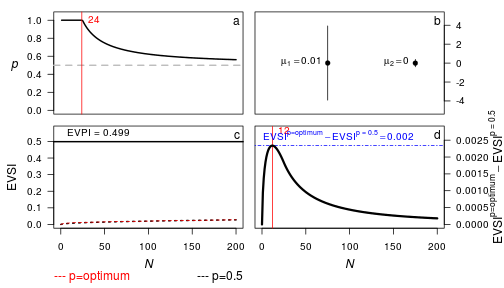
\includegraphics{figure/unnamed-chunk-3-1.png} \clearpage

We still allocate in the same way as before (a). The EVPI approaches its
theoretical maxmimum of 0.5. But the value of sample information
achievable for anything less than 200 samples is reduced to near zero
(c). The shape of the additional benefit from optimal allocation is the
same but the scale has reduced and the optimal value of N has increased
meaning more samples must be taken to maxmise the additional gain in
EVSI by using the optimal allocation vs the naive allocation of
\(p=0.5\) (d).

\textbf{\(\mu_1 \gg \mu_2, \sigma_1 \gg \sigma_2\)}

All other parameters still the same, but now with \(\mu_1=1\) much
greater than \(\mu_2\).

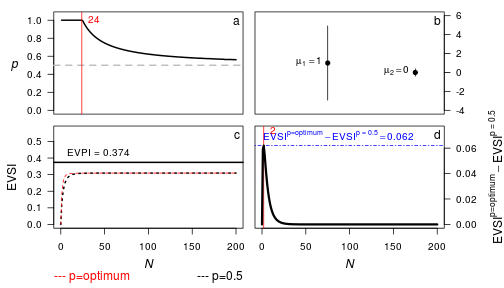
\includegraphics{figure/unnamed-chunk-4-1.png} \clearpage

Still same optimal allocation (a). EVPI reduced as we start already more
certain that \(A_1\) is a better asset than \(A_2\). The return on
investing in each additional sample diminishes quicker and sooner as
EVSI asymptotes at nearer EVPI (c). The additional benefit in EVSI seen
by sampling optimally has increased by peaks earlier at \(N=2\) (d).

\textbf{\(\mu_1 > \mu_2, \sigma_1 > \sigma_2\)}

Resetting \(\mu_1\) now we examine what happens when \(\sigma_1\) is
double \(\sigma_2\).

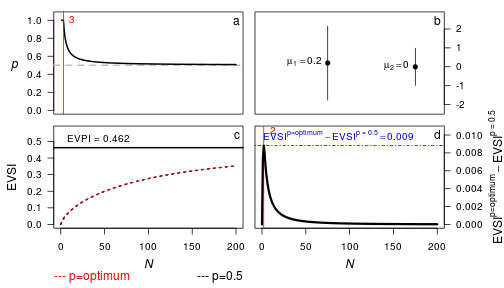
\includegraphics{figure/unnamed-chunk-5-1.png} \clearpage

The optimal allocation has the same shape as before but now we allocate
sampling to asset \(A_2\) sooner than before. Now if we take more than 3
samples we will allocate an increasing amount of them to asset \(A_2\)
(a). The EVPI has been reduced as we have started off more certain that
\(A_1\) is greater \(A_2\) (c). There is less advantage to sampling
optimally rather than the naive allocation but the point at which the
additional benefit in EVSI peaks is at higher \(N\) (\(N=2\)) than when
\(\sigma_1\) was much more than \(\sigma_2\) (d).

\textbf{\(\mu_1 > \mu_2, \sigma_1 = \sigma_2\)}

Now increase the precision of \(c_1\) so that \(\sigma_1 = \sigma_2\).

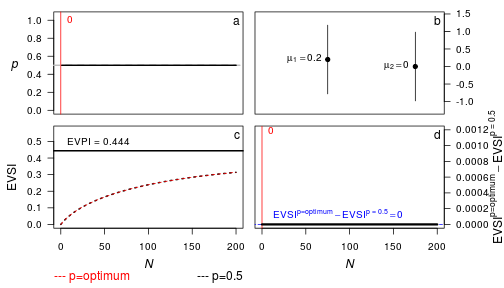
\includegraphics{figure/unnamed-chunk-6-1.png} \clearpage

Now the optimal allocation is to just allocate evenly between the assets
(i.e., the naive allocation is now optimal and there is effectively no
advantage to optimize) (a). The allocation is still insentive to the
value of \(\mu_1\) and the value of \(\sigma\)'s. Decreasing the prior
precisions increases EVPI, and with it the point at which EVSI vs \(N\)
asymptotes, but without changing the rate EVPI increases with \(N\).
Increaseing the value of \(\mu_1\) decreases EVPI (but less sensitively
than changing the precision) and also increases the rate at which EVPI
vs \(N\) approaches EVPI (c).

\textbf{\(\mu_1 > \mu_2, \sigma_1 \ll \sigma_2\)}

Returning to the original paramterisation now reverse the prior
precisions so that \(\tau^\prime_a\) is much greater than
\(\tau^\prime_b\).

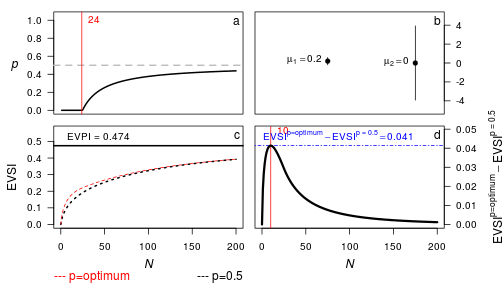
\includegraphics{figure/unnamed-chunk-7-1.png} \clearpage

The allocation is the same but now reflected so that we still allocate
to the asset with more uncertainty (a). This applies no matter what the
other parameter values are (i.e., the problem is symetrical).

\captionsetup{labelformat=default}
